\newpage
\section{Contexte technique}
Nous allons maintenant aborder les différentes notions au cœur du sujet du stage en commençant par définir les concepts de base de la virtualisation. 
Ensuite, nous allons définir la migration dans le contexte des machines virtuelles ainsi que quelques types de migration qui sont définis dans la littérature.
Enfin, nous traiterons le processus de migration de machine virtuelle qui est mis en place dans QEMU.

\subsection{Virtualisation}
Nous allons maintenant aborder les principaux concepts de la virtualisation.
Dans un premier temps, nous allons définir la virtualisation, les hyperviseurs et nous évoquerons les différentes solutions existantes ainsi que leurs caractéristiques.
Ensuite, nous découvrirons la combinaison QEMU et KVM.
Enfin, nous détaillerons la pile de virtualisations dans le cas d'une virtualisation à l'aide de QEMU et KVM.

\begin{description}
    \item[La virtualisation] est une technologie qui consiste à faire cohabiter plusieurs systèmes d'exploitation.
    Elle permet ainsi d'exécuter un ou plusieurs systèmes d'exploitation sur une même machine qui se comportent comme des ordinateurs complets.
    La virtualisation nous garantit aussi l'isolation des OS et ainsi en cas de panne (logiciel) d'un des deux systèmes, l’autre n’en sera pas impacté.

    Il existe deux principales techniques de virtualisation qui peuvent être mises en place par le biais de respectivement un hyperviseur de type I et II :

    \item[Un hyperviseur] parfois appelé moniteur de machine virtuelle (VMM), a pour but de gérer l’accès aux ressources physiques par les systèmes d’exploitation invités.
    L'hyperviseur traite les ressources (CPU, mémoire et stockage) comme un pool qui peut être facilement réaffecté entre les machines virtuelles.

    \item[Un hyperviseur de type I] interagit directement avec le matériel du système ; il n'a pas besoin d'un système d'exploitation hôte.
    Il est mis en place directement sur un système bare metal.
    Les hyperviseurs de type 1 sont également appelés hyperviseurs Bare Metal, Embedded ou Native.\cite{kvmbook}
    C'est une solution de virtualisation complète, car elle permet d'utiliser les extensions de virtualisation matérielle Intel VT ou AMD-V par exemple.


    \item[Un hyperviseur de type II] est exécuté en userland (sur système d'exploitation hôte).
    Le principal avantage des hyperviseurs de type 2 est la large gamme de supports matériels, car le système d'exploitation hôte sous-jacent contrôle l'accès au matériel.
    Les hyperviseurs de type 2 sont également appelés hyperviseurs hébergés. \cite{kvmbook}
    \end{description}



\subsubsection{Choix d'un hyperviseur : QEMU}
QEMU est un émulateur de machine, il permet d'effectuer la virtualisation du matériel.
Tous les périphériques que le système d'exploitation invité voit, comme un clavier, une souris, une carte réseau, etc. sont des instances de code dans QEMU.
Beaucoup de ces périphériques sont basés sur les spécifications publiées pour le matériel physique disponible.
Les systèmes d'exploitation invités peuvent reconnaître ces périphériques grâce aux pilotes qui leur sont fournis.
QEMU peut fonctionner seul et émuler toutes les ressources de la machine virtuelle, son émulation logicielle le rend cependant extrêmement lent.

En plus d'imiter le matériel réel, QEMU crée également certains périphériques écrits spécifiquement pour les cas d'utilisation de la virtualisation.
Dans le cas de la combinaison QEMU/KVM, le framework virtio est utilisé pour créer ces périphériques.
Nous avons par exemple un périphérique réseau virtio-net, un périphérique bloc virtio-blk et ainsi de suite.
Les périphériques paravirtualisés ont l'avantage d'être conçus avec la virtualisation en tête, ils sont donc généralement plus rapides et plus faciles à gérer que l'émulation de périphériques réels.

Pour son fonctionnement, QEMU utilise plusieurs services du noyau Linux de l'hôte, comme l'utilisation des API KVM par exemple.

KVM est un hyperviseur de type 1 qui s'insère sous forme d'un module au noyau Linux pour le convertir en un hyperviseur.
KVM délègue la gestion de la mémoire, l'ordonnancement des processus, etc. au noyau Linux.
Cela signifie que toute amélioration du côté de Linux profite immédiatement à l'hyperviseur.

KVM expose son API à l'espace utilisateur via des ioctls, c'est par ce biais que QEMU utilise ses services.

Comme mentionné précédemment, l'émulation logiciel de QEMU le rend extrêmement lent. 
Pour surmonter ce problème, QEMU permet d'utiliser KVM afin de pouvoir utiliser les extensions de virtualisation du CPU physique.
QEMU s'exécute dans l'espace utilisateur et effectue une émulation matérielle virtuelle, tandis que KVM s'exécute dans l'espace noyau (hyperviseur de type 1), qui permet à un programme de l'espace utilisateur d'accéder aux fonctions de virtualisation matérielle des processeurs.


\subsubsection{Pile de virtualisation}
Les utilisateurs interagissent avec les machines virtuelles via l'une des nombreuses interfaces disponibles, comme virt-manager ou oVirt.
Ces logiciels interagissent à leur tour avec libvirt, qui fournit une API neutre vis-à-vis de l'hyperviseur pour gérer les machines virtuelles.

Pour les machines virtuelles QEMU/KVM, libvirt dialogue avec QEMU en utilisant les API fournies par QEMU.
Chaque machine virtuelle créée sur un hôte possède sa propre instance QEMU.
L'invité est exécuté dans le cadre du processus QEMU et chaque vCPU invité est vu comme un thread séparé dans les sorties top(1) et ps(1) de l'hôte.

Par la suite, QEMU s'interface avec Linux, en particulier le module KVM dans Linux, pour exécuter directement les machines virtuelles sur le matériel physique. 

\begin{figure}[H]
    \centering
    \includegraphics[scale=0.5]{include/pile.png}
    \caption{Représentation de la pile de virtualisation}
\end{figure}



\subsection{Techniques de migration}
En virtualisation, la migration de machines virtuelles consiste à déplacer l'état et les données d'une machine virtuelle, d'un hôte physique à un autre.
C'est une technique largement répandue au sein des centres de données des fournisseurs afin de gérer la répartition de charge et faire de la consolidation des serveurs.

La migration du contenu de la mémoire d'une VM d'un hôte physique à un autre peut être abordée de différentes manières.
Cependant, lorsqu'une VM exécute un service actif, il est important que ce transfert s'effectue d'une manière à minimiser le temps d'arrêt et le temps total de migration.

Le temps d'arrêt est la période pendant laquelle le service est indisponible parce qu'il n'y a pas d'instance de la VM en cours d'exécution ; cette période sera directement visible pour les clients de la VM en tant qu'interruption de service.

Le temps total de migration est la durée entre le moment où la migration est lancée et le moment où la VM originale peut potentiellement être mise hors service pour maintenance, mise à niveau ou réparation.

Il est plus facile de considérer les compromis entre ces exigences en généralisant le transfert de mémoire en trois phases :
\begin{description}
    \item[Phase de push]
        La VM source continue de fonctionner pendant que certaines pages sont envoyées à travers le réseau vers la nouvelle destination.
        Pour garantir la cohérence, les pages modifiées pendant ce processus doivent être envoyées à nouveau.
    \item[Phase de Stop-and-copy]
        La VM source est arrêtée, les pages sont copiées sur la VM de destination, puis la nouvelle VM est démarrée.
    \item[Phase de pull]
        La nouvelle VM s'exécute et, si elle accède à une page qui n'a pas encore été copiée, cette dernière est envoyée à travers le réseau depuis la VM source.
\end{description}

Bien que l'on puisse imaginer un schéma intégrant les trois phases, la plupart des solutions pratiques n'en retiennent qu'une ou deux. 
Deux techniques de migration de machines virtuelles existent:

\subsubsection{Migration à froid (non-live)}
La migration à froid est la stratégie la plus basique, il est cependant nécessaire de mettre la machine virtuelle hors tension afin de copier l'état de sa mémoire sur l'hôte cible.
Cette méthode a pour avantage de n'impliquer aucune erreur lors de la migration de la mémoire. En effet, la machine étant arrêtée tous les services ne sont plus disponibles et la mémoire ne sera pas modifiée par des processus.
Une fois migrée, la machine virtuelle reprendra son activité dans le même état que lorsqu'elle s'est arrêtée.
Elle comporte cependant un désavantage, à partir du moment où la machine est arrêtée, les services fonctionnant sous celle-ci ne seront plus disponibles durant toute la durée de la migration.
Cela pose évidemment des problèmes majeurs pour des applications nécessitant une haute disponibilité.
De plus, la mémoire étant transférée entièrement sur l'hôte cible, la migration à froid provoque un ralentissement du réseau. 

\subsubsection{Migration à chaud (live)}
La migration à chaud consiste à déplacer une machine virtuelle d'une machine hôte vers une autre machine sans la mettre à l'arrêt. 
Durant la migration, l'invité peut continuer d'utiliser la machine sans aucune différence.
Les connexions réseau restent actives et les applications continuent de fonctionner pendant le transfert de la machine virtuelle.
Cela signifie que de nombreuses variables entrent en jeu : bande passante du réseau, latence du réseau, disponibilité du stockage, etc.

Il y a une petite fenêtre pendant laquelle l'invité doit être arrêté pour que le nouvel hyperviseur prenne le relais et commence à exécuter l'invité.
Cela peut entraîner une dégradation des performances des applications de l'invité, et c'est la seule exposition de l'invité au processus de migration.

La migration à chaud est également appelée migration en direct.

Les deux types de migrations à chaud les plus connues sont :

\paragraph*{La migration pré-copie}
Elle combine une phase de push itérative suivie avec une phase d'arrêt et de copie généralement très courte.
Par \texttt{itératif}, nous entendons que la pré-copie se produit par cycles, dans lesquels les pages à transférer pendant le cycle sont celles qui ont été modifiées par des processus pendant le cycle précédent.

KVM expose à l'espace utilisateur une fonctionnalité gardant la trace des pages mémoires de l'invité qui ont été modifiées depuis la fois que celles-ci ont été demandées. 
Cette fonctionnalité permet notamment à QEMU d'envoyer uniquement les pages utilisées pendant le processus de migration.
La possibilité pour l'espace utilisateur, comme QEMU, de savoir quelles pages ont été modifiées depuis la dernière fois que ces données ont été demandées permet d'envoyer uniquement les pages sales.

Lors de la première phase de la migration, toutes les pages seront marquées comme sales.
La première itération transférera ainsi toutes les pages de mémoire.
Si les pages sales restantes calculées tombent sous la ligne de flottaison, la machine virtuelle peut être suspendue et les pages sales restantes ainsi que l'état des périphériques seront migrés en une seule fois.

Lorsque la mémoire de la machine virtuelle change fortement, le nombre des pages sales ne peuvent jamais descendre en dessous de la ligne de flottaison, ce qui implique que la migration ne peut donc jamais être achevée.
En d'autres termes, plus le nombre d'écritures en mémoire est important, plus la migration aura du mal à converger. 

\paragraph*{La migration on-demand (post-copie)}
En réponse aux problèmes ci-dessus, la méthode post-copie a été proposée.

Cette migration procède dans un premier lieu au transfert des structures de données essentielles vers la destination.
La VM de destination est ensuite démarrée, le reste des données est alors transféré depuis la machine source vers la machine virtuelle destinatrice à l'aide d'une combinaison de 4 techniques :
\begin{description}
    \item[Demand-paging] permet à l'hôte cible de demander une page mémoire manquante (Page fault) à l'hôte source, cette méthode implique inévitablement un ralentissement du système de par la lenteur du réseau.
    \item[Active-push] permet à l'hôte source d'envoyer à la cible les pages mémoire manquantes qui n'ont pas encore été demandées par l'hôte cible de manière pro-active.
    \item[Pre-paging] est un système permettant à l'hôte source de prédire la prochaine page fautive sur l'hôte cible en fonction des défauts de page récents.
    \item[Dynamic self balooning] permet quant à lui de réduire le nombre de transferts des pages non allouées.
\end{description}

La copie de pages sales du modèle pré-copie doit être terminée avant le démarrage de la machine virtuelle de destination, tandis que la copie de pages sales du modèle post-copie se poursuivra même après la reprise de la VM.

Cela permet de réduire considérablement le temps d'arrêt.
Dans la pratique, les performances après la migration sont susceptibles d'être dégradées jusqu'à ce qu'un ensemble considérable de pages ait été transférée.
Durant la migration, la machine virtuelle fera des erreurs sur une grande partie de ses accès à la mémoire, chacun d'entre eux initiant un transfert synchrone sur le réseau.

La migration en post-copie permet à la migration en direct de s'achever en un temps fini, indépendamment de la charge de la mémoire de la VM, ce qui constitue un outil fiable pour gérer la charge du serveur entre les hôtes.

Le principal inconvénient du mécanisme de post-copie est que toute interruption du réseau entraîne la perte de la VM.

\paragraph*{Migration hybride}
Le mécanisme de post-copie peut être utilisé pour aider la migration pré-copie.
En tant que telle, l'approche n'est ni purement pré-copie ni purement post-copie, mais un hybride qui combine les aspects des deux.
L'approche hybride est principalement utilisé lorsque la VM peut être migrée avec succès avec la technique de pré-copie, sans risque de perdre une instance en cas de défaillance réseau.

Le passage à la post-copie peut être effectué à tout moment s'il est conclu que la migration prend trop de temps et qu'elle ne convergera probablement pas dans un délai raisonnable.
Elle peut donc être utilisée comme solution de repli dans les scénarios où la VM est bloquée dans un état de migration en raison d'une forte activité mémoire.

Le principal inconvénient reste le même que pour la méthode post-copie, toute interruption du réseau entraîne la perte de la VM.

La combinaison de ces solutions de migration en direct offre le potentiel d'une gestion de la charge beaucoup plus fluide et flexible.


\begin{figure}[H]
    \centering
    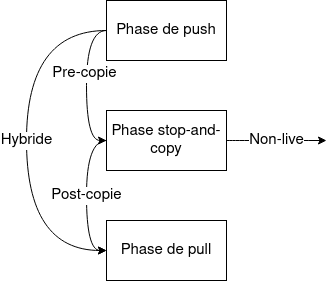
\includegraphics[scale=0.5]{include/typemig.png}
    \caption{Représentation des différents types de migration}
\end{figure}

\subsection{Migration dans QEMU}
Nous allons maintenant aborder les différentes structures utilisées dans le cadre des migrations de machines virtuelles.
Ensuite, nous allons définir le protocole d'échange utilisé par les deux bouts de la migration.
Par la suite, nous décrirons le processus de migration de machine virtuelle avec les différents algorithmes qui sont mis en place.
Enfin, nous aborderons le sujet de la migration du disque.

\subsubsection{Structures de données dans QEMU}

Lors de la migration des objets, on peut distinguer deux types de périphériques :
\begin{description}
\item[Itératifs] concerne les périphériques avec un grand volume de données (RAM, disques ...).
\item[Non-itératifs (la plupart)] les données sont envoyées lorsque les CPUs sont stoppés
\end{description}

Chaque machine virtuelle a la capacité de sauvegarder un état complet et restaurable, y compris son vCPU, sa RAM et ses périphériques.

\subsubsection*{SaveState et SaveStateEntry}
Une structure de donnée de type \texttt{SaveStateEntry} est allouée pour chaque objet qui doit être migré.

Le principe de la migration des devices est de transférer chaque \texttt{SaveStateEntry} vers la machine de destination. 
Les informations contenues dans \texttt{SaveStateEntry} peuvent être des pages mémoire ou l'état des devices, on peut les distinguer par la variable \texttt{is\_ram}. 
Pour la machine virtuelle en cours d'exécution, ces informations peuvent changer à tout moment.

Les \texttt{SaveStateEntry} sont insérées dans une liste globale \texttt{savevm\_state} de type \texttt{SaveState}. 
\begin{figure}[H]
    \centering
    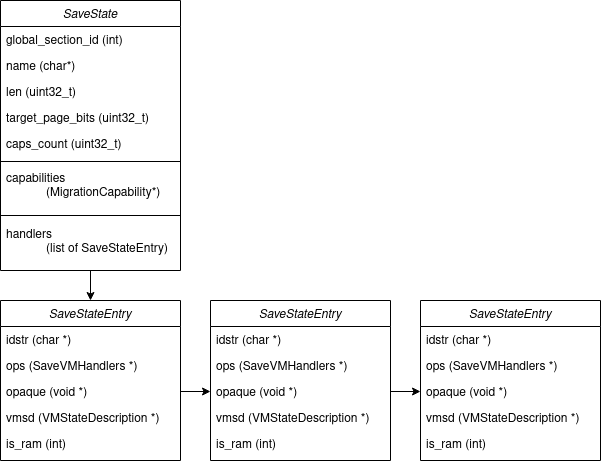
\includegraphics[width=\textwidth]{include/savestate.png}
    \caption{Schéma des structures SaveState et SaveStateEntry}
\end{figure}

Les opérations de migrations de chaque objet peuvent être encodées de deux manières différentes :
\begin{description}
\item[Par une structure de type \texttt{SaveVMHandlers}] contenue dans le champs `ops` du \texttt{SaveState} qui contient un ensemble de pointeurs de fonctions utilisé au cours du processus de migration.
\item[Par une structure de type \texttt{VMStateDescription}] contenue dans le champs `vmsd` qui permet d'encoder de manière générique n'importe quel périphérique en structure de données en C.
\end{description}

\subsubsection*{SaveVMHandlers (Legacy)}
\texttt{SaveVMHandlers} modélise les opérations à effectuer pour migrer un objet, ces fonctions s'occupent d'écrire et de récupérer dans une zone mémoire (opaque) l'intégralité de l'état du périphérique.
Chaque périphérique doit enregistrer au moins deux fonctions, une pour sauvegarder l'état et une autre pour le charger.
Voici un exemple d'initialisation de la structure pour la migration de la RAM.

\begin{lstlisting}[caption={Exemple d'une structure de donnée SaveVMHandlers},captionpos=b]
static SaveVMHandlers savevm_ram_handlers = {
    .save_live_setup = ram_save_setup,
    .save_live_iterate = ram_save_iterate,
    .save_live_complete_postcopy = ram_save_complete,
    .save_live_complete_precopy = ram_save_complete,
    .save_live_pending = ram_save_pending,
    .load_state = ram_load,
    .cleanup = ram_migration_cleanup,
};
\end{lstlisting}

\subsubsection*{VMStateDescription}
\texttt{VMStateDescription} décrit un VMState, il permet d'encoder de manière générique un ensemble de données à envoyer.
En d'autres termes", \texttt{VMState} est l'état du périphérique dans le modèle de périphérique QEMU.
Chaque état de périphérique a une structure.
La fonction principale d'un \texttt{VMStateDescription} est d'aider QEMU à juger pendant la migration, quels membres de la structure \texttt{VMState} doivent être migrés.
Pour qu'un device puisse être inclut dans une sauvegarde elle doit implémenter l'interface \texttt{VMStateDescription}, qui va contenir tous les champs nécessaires qui devrons être restaurés.
Prenons l'exemple de l'implémentation de IOMMU (Input-Output Memory Management Unit) :

\begin{lstlisting}[caption={Exemple d'une structure de donnée VMStateDescription},captionpos=b]
static const VMStateDescription vtd_vmstate = {
    .name = "iommu-intel",
    .version_id = 1,
    .minimum_version_id = 1,
    .priority = MIG_PRI_IOMMU,
    .post_load = vtd_post_load,
    .fields = (VMStateField[]) {
        VMSTATE_UINT64(root, IntelIOMMUState),
        VMSTATE_UINT64(intr_root, IntelIOMMUState),
        VMSTATE_UINT64(iq, IntelIOMMUState),
        VMSTATE_UINT32(intr_size, IntelIOMMUState),
        VMSTATE_UINT16(iq_head, IntelIOMMUState),
        [ . . . ]
        VMSTATE_END_OF_LIST()
    }
};
\end{lstlisting}

Dans cet exemple, \texttt{VMStateDescription} expose tous les registres internes de l'IOMMU afin qu'ils soient automatiquement sauvegardés et restaurés lors de la migration.
Cette méthode est générique et ne nécessite pas d'écriture de fonction qui permet de sauvegarder ou de restaurer les données.


\texttt{VMStateDescription} contient un tableau de champs, chaque élément étant une structure \texttt{VMStateField}.
Chaque champ contient plusieurs éléments, dont le nombre est déterminé par \texttt{num/num\_offset}, et sa taille est déterminée par \texttt{size/size\_offset}.
La position de départ des éléments est déterminée par offset, dans l'espace pointé par le pointeur opaque.

\texttt{VMStateDescription} n'existe pas seul, mais fait partie de \texttt{SaveStateEntry}.
Mais toutes les structures \texttt{SaveStateEntry} n'ont pas vmsd.
Par exemple, dans les \texttt{SaveStateEntry} de "ram" et "block" le vmsd n'est pas disponibles, il est remplacé par des routines \texttt{SaveVMHandlers}. 
\begin{figure}[H]
    \centering
    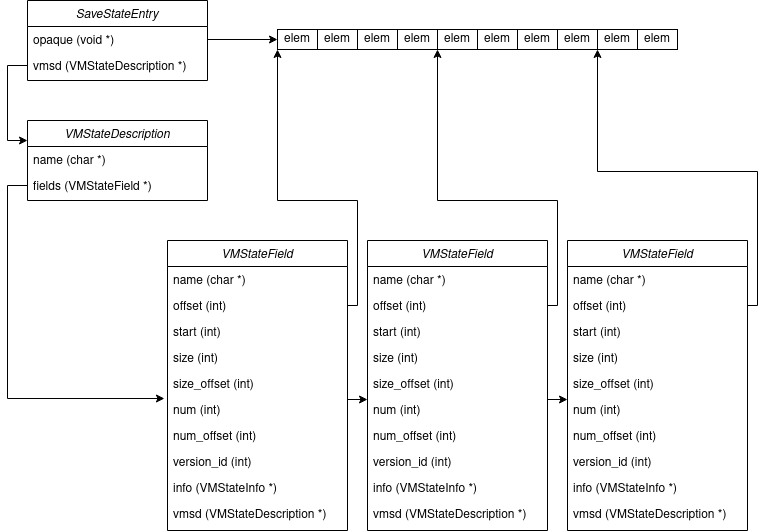
\includegraphics[width=\textwidth]{include/VMDescription.png}
    \caption{Schéma de la structure VMStateDescription}
\end{figure}



\subsubsection{Protocole d'échange}
Tout échange d’informations repose nécessairement sur un ensemble de conventions partagées entre l'émetteur et le destinataire d'un message.
Il faut que l'un et l'autre sachent notamment à quel moment commence la communication, avec quelle procédure (pour l'interprétation des données) et à quel moment elle se termine.


Il existe différents protocoles de transport qui peuvent être utilisés pour le transport du flux :
\begin{description}
    \item[tcp] utilise les sockets tcp.
    \item[unix] utilise les sockets unix.
    \item[exec] utilise les standards stdin/stdout à travers un processus.
    \item[fd] utilise un descripteur de fichier déjà ouvert.
    \item[rdma] utilise le protocole RMDA, ce qui permet de réduire le stress sur le CPU.
\end{description}

Habituellement, la migration de la machine virtuelle contrôlée par libvirt utilise la migration fd, qui est un moyen pratique de migration.
Le descripteur de fichier est ouvert par l'application de plus haut niveau (libvirt), et QEMU est seulement responsable de l'envoi de données au descripteur.


Sur QEMU, le protocole d'échange envoie les données sous forme d'objet au sein d'un flux.
Chaque objet peut être envoyé en de multiples parties encapsulées au sein de sections délimitées par des constantes numériques afin de multiplexer l'envoi de parties d'objets.

\subsubsection*{QEMU Section}

La migration de mémoire de QEMU prend la section comme unité, et toutes les informations migrées sont encapsulées dans des sections pour être écrites dans le flux de sortie. 

Le format d'une section est indiqué ci-dessous. 

\begin{figure}[H]
    \centering
    \begin{tabular}{|c | c|} 
        \hline
        Type & Specifique au type\\ 
        \hline
    \end{tabular}
    \caption{Représentation du format d'une section QEMU}

\end{figure}

Le premier octet est le champ de type.
Le contenu suivant varie selon les sections.

Voici les différentes sections qui interviennent lors de la migration d'une VM :

\begin{figure}[H]
    \centering
    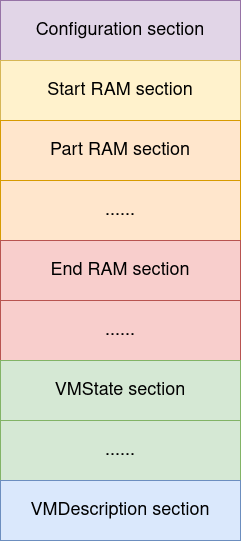
\includegraphics[scale=0.4]{include/section.png}
    \caption{Liste des différentes sections utilisées lors de la migration}
\end{figure}

\begin{description}
    \item[Configuration section]
    Cette section de la migration est spéciale.
    Il s'agit de la section de configuration.
    Comme son nom l'indique, sa fonction est de configurer la migration.
    Il s'agit d'une section de l'état des périphériques, indiquant le type de machine de la machine virtuelle source.
    Lorsque la destination analyse la section, elle compare le type de machine.
    Si les champs ne sont pas les mêmes, la migration n'est pas autorisée, ce qui limite la migration des machines virtuelles ayant des types de machine différents à la source et à la destination.
    \item[RAM start section]
    Cette section est également spéciale.
    Il s'agit des métadonnées de toute la mémoire migrée, y compris la taille totale de la mémoire de tous les \texttt{SaveStateEntry}, ainsi que la longueur totale des \texttt{RAMBlock} pointé par chaque sous-ensemble de mémoire \texttt{SaveStateEntry}.

    \item[RAM part section]
    Cette section correspond aux données de la RAM.

    \item[VMState section]
    Cette section décrit tous les champs d'état du périphérique migrés.

    \item[VMDescription section]
    Cette section est constituée d'une description JSON du contenu à des fins d'analyse uniquement.

\end{description}

\subsubsection{Processus de migration}

\paragraph*{Côté source}
Le début de la migration de la mémoire se trouve dans \texttt{migration\_thread()} et est divisé en 4 étapes : 

\subparagraph*{Initiation de la migration}
Dans l'étape d'initiation de la migration, l'en-tête de migration de la mémoire est envoyée pour marquer le début de la migration.
Les informations de l'en-tête de migration sont alors envoyées ainsi que le magic number et la version.
Cette section est configurée comme une information facultative, en fonction du type de machine.
\begin{lstlisting}[caption={Code responsable de la phase d'initiation},captionpos=b]
qemu_savevm_state_header()
{       
    qemu_put_be32(f, QEMU_VM_FILE_MAGIC);
    qemu_put_be32(f, QEMU_VM_FILE_VERSION);
            
    if (migrate_get_current()->send_configuration) {
        qemu_put_byte(f, QEMU_VM_CONFIGURATION);
        vmstate_save_state(f, &vmstate_configuration, &savevm_state, 0);
    }       
} 
\end{lstlisting}

\subparagraph*{Préparation de la migration}
Il existe une liste pour les pages de mémoire qui doivent être transférées \texttt{ram\_list.blocks}. 
L'étape de préparation de la migration fait principalement deux choses :
\begin{enumerate}
    \item Marquer toute la mémoire (les rajouter dans \texttt{ram\_list.blocks}).
    \begin{lstlisting}[caption={Différentes fonctions d'initialisation de la bitmap},captionpos=b]
        ram_init_all
            ram_init_bitmaps
                ram_list_init_bitmaps()
                memory_global_dirty_log_start()
                migration_bitmap_sync_precopy(rs)
    \end{lstlisting}

    \item Envoyer les noms et tailles de toutes les pages migrés.
    \begin{lstlisting}[caption={Code responsable de l'envoie des nom et tailles des pages migrés},captionpos=b]
        RAMBLOCK_FOREACH_MIGRATABLE(block) {
            qemu_put_byte(f, strlen(block->idstr));
            qemu_put_buffer(f, (uint8_t *)block->idstr, strlen(block->idstr));
            qemu_put_be64(f, block->used_length);
        }
    \end{lstlisting}
\end{enumerate}

\subparagraph*{Copie de la migration}
La phase de copie de migration consiste simplement à copier les données de la mémoire vers la destination.
Le processus est le suivant :
la dirty bitmap est parcouru afin de trouver une page qui a été changé depuis la dernière itération pour la transférer vers la destination.
\begin{lstlisting}[caption={Code responsable de la phase de copie},captionpos=b]
ram_save_iterate()
{
  	pages = ram_find_and_save_block(rs, false)
    found = find_dirty_block(rs, &pss, &again)
    if (found) {
        pages = ram_save_host_page(rs, &pss, last_stage);
    }
}
\end{lstlisting}

\subparagraph*{Fin de la migration}
La toute première implémentation de la ligne de flottaison dans QEMU était plutôt simpliste : s'il restait 50 pages sales ou moins à migrer, nous passions à l'étape de fin.
Ou, lorsqu'un certain nombre d'itérations s'étaient écoulées sans que l'on ait progressé vers un nombre de pages sales inférieur à 50.

Cela a bien fonctionné au départ, cependant il a fallu ajouter plusieurs nouvelles contraintes.

Une mise à jour de QEMU à permis de changer quelques paramètres au code pour que les conditions de passage de l'étape de copie à celle de fin soient configurable par les administrateurs de l'hôte et de l'invité.

Les administrateurs invités peuvent spécifier le temps d'arrêt maximum acceptable.
Dans notre code de l'étape de copie, nous vérifions combien de pages sont modifiés (sales) à chaque itération par l'invité et combien de temps il faut pour transférer les pages à travers le réseau.
Cela nous permet de dresser une estimation de la bande passante du réseau.
En fonction de cette estimation et du nombre de pages sales de l'itération en cours, nous pouvons calculer le temps qu'il faudra pour transférer les pages restantes.
Si ce temps est dans la limite acceptable, nous passons à l'étape de fin.
Sinon, une nouvelle itération est faite. \cite{redhat}

À la fin de l'étape de migration, il y a trois phases principales : suspendre le processeur, copier la mémoire restante ainsi que les différents états des périphériques et copier l'état de la VM.

Le graphique ci-dessous montre les différentes sections envoyées dans chaque phase:
\begin{figure}[H]
    \centering
    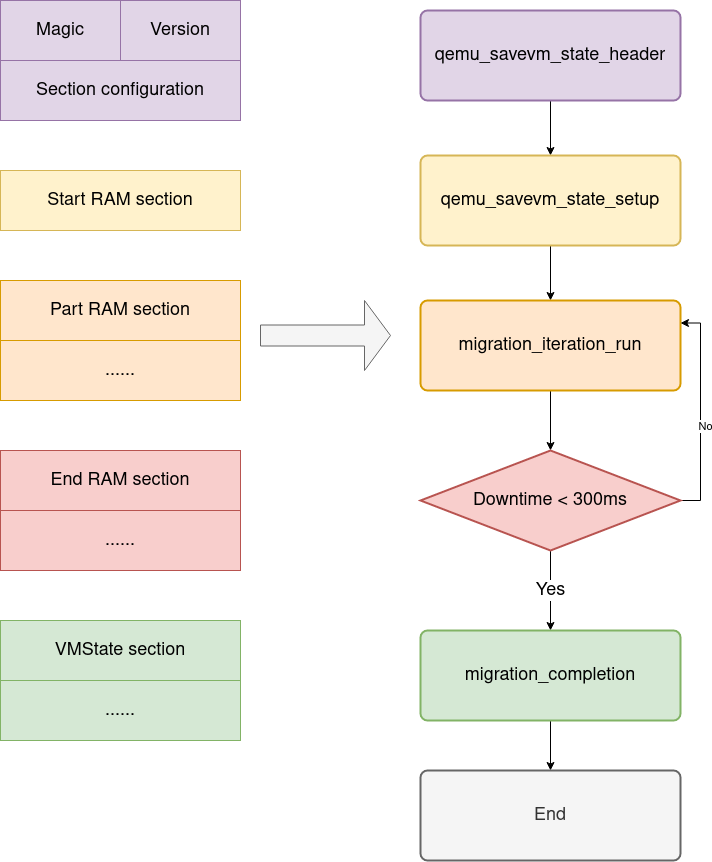
\includegraphics[scale=0.4]{include/summerize.png}
    \caption{Relation entre les différentes sections et les phases de la migration}
\end{figure}

\paragraph*{Côté destination}

Le processus central de la migration de destination est \texttt{qemu\_loadvm\_state()}, le processus est le suivant : 

\subparagraph*{Préparation de la migration}
Dans la phase d'initiation de la migration, les champs du magic number, de version et de configuration sont analysés et la fonction configuration est appelée en même temps. 
\begin{lstlisting}[caption={Code responsable de la phase de préparation},captionpos=b]

    /* magic */
    m = qemu_get_be32(f);

    /* version */
    v = qemu_get_be32(f);


    /* configuration section */
    if (migrate_get_current()->send_configuration)
        ret = vmstate_load_state(f, &vmstate_configuration, &savevm_state, 0);

\end{lstlisting}

\subparagraph*{Copie de la migration}
La logique principale de la copie de migration est dans \texttt{qemu\_loadvm\_state\_main}.
Dans cette fonction, le type de section est analysé à partir du flux.
Comme le format de la section est le même, la section peut être analysée de la même manière.
Les différents types de sections ont seulement une logique de traitement différente, comme ci-dessous : 
\begin{lstlisting}[caption={Code responsable de la phase de copie},captionpos=b]
qemu_loadvm_state_main()
{       
retry:
    while (true) {
    	/* section */
        section_type = qemu_get_byte(f);
          
        switch (section_type) {
        case QEMU_VM_SECTION_START:
        case QEMU_VM_SECTION_FULL:
            ret = qemu_loadvm_section_start_full(f, mis);
			[ . . .]
            break;
        case QEMU_VM_SECTION_PART:
        case QEMU_VM_SECTION_END:
            ret = qemu_loadvm_section_part_end(f, mis);
            [ . . .]
            break;   
        case QEMU_VM_COMMAND:
            ret = loadvm_process_command(f);
    		[ . . .]
            break;
        case QEMU_VM_EOF:
            /* This is the end of migration */
            goto out;
        default:
        [ . . .]
            goto out;
        }
    }
    [ . . .]
}

\end{lstlisting}

\subsubsection{Migration disque}
Il existe plusieurs fonctionnalités implémentées dans QEMU pour manipuler les périphériques de stockage et les données, alors que l'invité est en cours d'exécution.
\begin{description}
    \item[migrate -b] est la fonctionnalité traditionnelle de migration de disque dans qemu-kvm.
    Elle copie le contenu d'un périphérique de bloc dans le cadre du flux de migration en direct.
    Il s'agit d'une approche de pré-copie utilisant une dirty bitmap.

    \item[block-stream] peut être utilisé pour la migration pré et post-copie.
    Elle crée un nouveau fichier image qui utilise l'ancienne image disque comme fichier de sauvegarde.
    Le contenu du fichier de sauvegarde est copié dans la nouvelle image, à condition qu'aucun nouveau bloc n'a été écrit.
    Elle nécessite l'utilisation de NFS ou d'un autre mécanisme pour accéder à la fois à la nouvelle image et au fichier de sauvegarde en même temps.
    Cette méthode n'utilise pas le flux de migration en direct.

    \item[drive-mirror] le principe est de pré-copier le contenu du disque sur l'hôte de destination.
    Elle n'utilise pas de fichiers de sauvegarde, l'image de destination peut donc être de n'importe quel format d'image.
    Là encore, elle nécessite NFS ou un autre mécanisme pour accéder à la fois à la nouvelle image et à l'ancienne.
    Cette méthode n'utilise pas le flux de migration en direct.

    Un avantage de l'approche drive-mirror par rapport à block-stream est que la machine virtuelle peut continuer à s'exécuter sur l'ancienne image en cas de panne de courant ou de crash pendant la migration.
\end{description}


\subsubsubsection{Processus de migration du disque}
Nous allons nous intéresser à la migration traditionnelle (migrate -b) car c'est la seule qui utilise le même flux que la migration de la mémoire.
Dans ce cas, le disque est considéré comme un simple device, il utilise la même logique que la migration de la mémoire.
Il existe une structure \texttt{SaveVMHandlers} pour définir les routines qui permettent de migrer le contenue des blocs du disque.

\begin{lstlisting}[caption={SaveVMHandlers responsable de la migration du disque},captionpos=b]
static SaveVMHandlers savevm_block_handlers = {
    .save_setup = block_save_setup,
    .save_live_iterate = block_save_iterate,
    .save_live_complete_precopy = block_save_complete,
    .save_live_pending = block_save_pending,
    .load_state = block_load,
    .save_cleanup = block_migration_cleanup,
    .is_active = block_is_active,
};
\end{lstlisting}

\paragraph*{Côté source}
Nous allons maintenant définir les différentes phases de la migration du disque coté source.

\paragraph*{Préparation de la migration}
Cette phase permet d'initialiser toutes les structures de données qui vont être utilisées lors de la migration du disque.
Par la suite le même mécanisme de dirty bitmap est mis en place.
Au départ, tous les blocs sont marqués comme sale.

\begin{lstlisting}[caption={Code responsable de la phase de préparation},captionpos=b]
static int block_save_setup(){
    [ . . .]
    ret = init_blk_migration(f);
    [ . . .]
    /* start track dirty blocks */
    ret = set_dirty_tracking();
    [ . . .]
}
\end{lstlisting}


\subparagraph*{Copie de la migration}
Dans cette phase, QEMU commence à transférer les blocs de disque qui sont marqués comme sales.
Dans un premier temps, on commence par une phase pour transférer tous les blocs disque existants.
Puis on enchaîne par une phase Dirty qui permet de transférer seulement les blocs qui ont subi des écritures.

\begin{lstlisting}[caption={Code responsable de la phase de copie},captionpos=b]
static int block_save_iterate()
{
    [ . . .]
    /* control the rate of transfer */
    while (block_mig_state.read_done * BLK_MIG_BLOCK_SIZE <
           qemu_file_get_rate_limit(f) &&
           block_mig_state.submitted < MAX_PARALLEL_IO &&
           (block_mig_state.submitted + block_mig_state.read_done) <
           MAX_IO_BUFFERS) {

        if (block_mig_state.bulk_completed == 0) {
            /* first finish the bulk phase */
            if (blk_mig_save_bulked_block(f) == 0) {
                /* finished saving bulk on all devices */
                block_mig_state.bulk_completed = 1;
            }
        } else {
            /* Always called with iothread lock taken for
             * simplicity, block_save_complete also calls it.
             */
            qemu_mutex_lock_iothread();
            ret = blk_mig_save_dirty_block(f, 1);
            qemu_mutex_unlock_iothread();
        }
    }
    [ . . .]
}
\end{lstlisting}

\subparagraph*{Fin de la migration}
Le passage de la phase deux à la phase trois est la même que pour la migration de la mémoire.
Si le temps pour transférer les blocs restants est dans la limite acceptable, nous passons à l'étape de fin.
Dans cette phase, la machine virtuelle est gelée, et le transfert des derniers blocs dirty se fait.

\begin{lstlisting}[caption={Code responsable de la phase de fin},captionpos=b]
static int block_save_complete()
{
    [ . . .]
    /* we know for sure that save bulk is completed and
       all async read completed */
    [ . . .]
    do {
        ret = blk_mig_save_dirty_block(f, 0);
        if (ret < 0) {
            return ret;
        }
    } while (ret == 0);

    /* report completion */
    [ . . .]
}
\end{lstlisting}



\paragraph*{Côté destination}
La récupération des donnés côtés destination consiste en une phase décrite dans la fonction \texttt{block\_load()}.
Dans un premier temps, on récupère le nom du device et le numéro du secteur.
\begin{lstlisting}[caption={Code responsable de la récupération du nom du device et du numéro de secteur},captionpos=b]
    addr = qemu_get_be64(f);
       
    flags = addr & (BDRV_SECTOR_SIZE - 1);
    addr >>= BDRV_SECTOR_BITS;

    if (flags & BLK_MIG_FLAG_DEVICE_BLOCK) {
        /* get device name */
        len = qemu_get_byte(f);
        qemu_get_buffer(f, (uint8_t *)device_name, len);
        device_name[len] = '\0';
        blk = blk_by_name(device_name);
        [ . . .]
    }
\end{lstlisting}

Par la suite, on récupère les données pour mettre à jour le disque coté destination.
\begin{lstlisting}[caption={Code responsable de la récupération des données},captionpos=b]
    buf = g_malloc(BLK_MIG_BLOCK_SIZE);
    qemu_get_buffer(f, buf, BLK_MIG_BLOCK_SIZE);
\end{lstlisting}
